\documentclass[12pt,a4paper]{article}
\usepackage{amsmath,amscd,amsbsy,amssymb,latexsym,url,bm,amsthm}
\usepackage{epsfig,graphicx,subfigure}
\usepackage{enumitem,balance}
\usepackage{wrapfig}
\usepackage{appendix}
\usepackage{soul}
\usepackage{listings}
\usepackage{mathrsfs,euscript}
\usepackage[usenames]{xcolor}
\usepackage{hyperref}
\usepackage[vlined,ruled,linesnumbered]{algorithm2e}
\usepackage{fontspec}

\newtheorem{theorem}{Theorem}
\newtheorem{lemma}[theorem]{Lemma}
\newtheorem{proposition}[theorem]{Proposition}
\newtheorem{corollary}[theorem]{Corollary}
\newtheorem{exercise}{Exercise}
\newtheorem*{solution}{Solution}
\newtheorem{definition}{Definition}
\theoremstyle{definition}

\renewcommand{\thefootnote}{\fnsymbol{footnote}}

\newcommand{\postscript}[2]
 {\setlength{\epsfxsize}{#2\hsize}
  \centerline{\epsfbox{#1}}}

\renewcommand{\baselinestretch}{1.0}

\setlength{\oddsidemargin}{-0.365in}
\setlength{\evensidemargin}{-0.365in}
\setlength{\topmargin}{-0.3in}
\setlength{\headheight}{0in}
\setlength{\headsep}{0in}
\setlength{\textheight}{10.1in}
\setlength{\textwidth}{7in}
\makeatletter \renewenvironment{proof}[1][Proof] {\par\pushQED{\qed}\normalfont\topsep6\p@\@plus6\p@\relax\trivlist\item[\hskip\labelsep\bfseries#1\@addpunct{.}]\ignorespaces}{\popQED\endtrivlist\@endpefalse} \makeatother
\makeatletter
\renewenvironment{solution}[1][Solution] {\par\pushQED{\qed}\normalfont\topsep6\p@\@plus6\p@\relax\trivlist\item[\hskip\labelsep\bfseries#1\@addpunct{.}]\ignorespaces}{\popQED\endtrivlist\@endpefalse} \makeatother

\begin{document}
\noindent

%========================================================================
\noindent\framebox[\linewidth]{\shortstack[c]{
\Large{\textbf{Lab02-Divide and Conquer}}\vspace{1mm}\\
CS214-Algorithm and Complexity, Xiaofeng Gao, Spring 2021.}}
\begin{center}

\footnotesize{\color{blue}$*$ Name:\underline{\quad   Haoyi You  \quad  }\quad Student ID:\underline{\quad 519030910193 \quad} \quad Email: \underline{\quad yuri-you@sjtu.edu.cn \quad}}
\end{center}

\begin{enumerate}
\item
    \textit{Recurrence examples.} Give asymptotic upper and lower bounds for $T(n)$ in each of the following recurrences. Assume that $T(n)$ is constant for sufficiently small $n$. Make your bounds as tight as possible.
\begin{enumerate}
	\item $T(n)=4 T(n / 3)+n \log n$
	\item $T(n)=4 T(n / 2)+n^{2} \sqrt{n}$
	\item $T(n)=T(n-1)+n$	
	\item $T(n)=2T(\lfloor \sqrt n\rfloor)+\log n$
\end{enumerate}
\begin{solution}
    We formalize the recurrence equation as below:
    \begin{equation}
        T(n)=aT(n/b)+f(n)
    \end{equation}
    Here $n/b$ can be replaced be $\lfloor n/b\rfloor$ or $\lceil n/b\rceil$ 
	\begin{enumerate}
	\item $a=4,b=3,log_b a=log_34,f(n)=n log n\le n^{log_34}$,so that $T(n)=\Theta(n^{log_3 4})$
	\item $a=4,b=2,log_b a=log_24=2,f(n)=n^{2.5}\ge n^2$,so that $T(n)=\Theta(n^{2.5})$
	\item $T(n)=T(n-1)+n=T(n-2)+n+n-1=...=T(1)+\sum_{i=2}^{n}i=\Theta(n^2)$
	\item let $n=2^z,T(n)=S(z)$,we can change the equation to
	\begin{equation}
	    S(z)=2*T(\lfloor\sqrt{2^z}\rfloor)+z=2*T(\lfloor2^{z/2}\rfloor)+z=2*S(\lfloor z/2\rfloor)+z
	\end{equation}
	now $a=2,b=2,log_b a=1,f(z)=\Theta(z)$, so that $T(n)=S(logn)=\Theta(z log z)=\\\Theta(logn*log(logn))$
\end{enumerate} 
\end{solution}
\item
\textit{Divide-and-conquer.} Given an integer array $A[1..n]$ and two integers $lower \le upper$, design an algorithm using \textbf{divide-and-conquer} method to count the number of ranges $(i,j)$ ($1 \leq i \leq j \leq n$) satisfying
$$
    lower \leq \sum_{k=i}^{j}{A[k]} \leq upper.
$$
\textbf{Example:}

Given $A = [1,-1,2]$, $lower = 1$, $upper = 2$, return 4.

The resulting four ranges are $(1,1)$, $(3,3)$, $(2,3)$ and $(1,3)$.

\begin{enumerate}
\item
Complete the implementation in the provided C/C++ source code {\color{blue}(The source code \emph{Code-Range.cpp} is attached on the course webpage)}.
\item
Write a recurrence for the running time of the algorithm and solve it by recurrence tree {\color{blue}(You can modify the figure sources \emph{Fig-RecurrenceTree.vsdx} or \emph{Fig-RecurrenceTree.pptx} to illustrate your derivation)}.
\item
Can we use the Master Theorem to solve the recurrence above? Please explain your answer.
\end{enumerate}
\begin{solution}
~\par
\begin{enumerate}
\item Please refer to the appendix 1.
\item Assume the complexity is $T(n)$,where $n$ is the length of the array.In one n-length array recursion,it generates two half length recursion. Besides,each binary search costs $logn$ operations and there are $n$ binary searches.Also the sort function costs $O(nlogn)$ operations.
From the analysis above we can get:
\begin{equation}
    T(n)=2*T(n/2)+O(nlogn)
    \label{recursion}
\end{equation}
\begin{figure}[htbp]
    \centering
    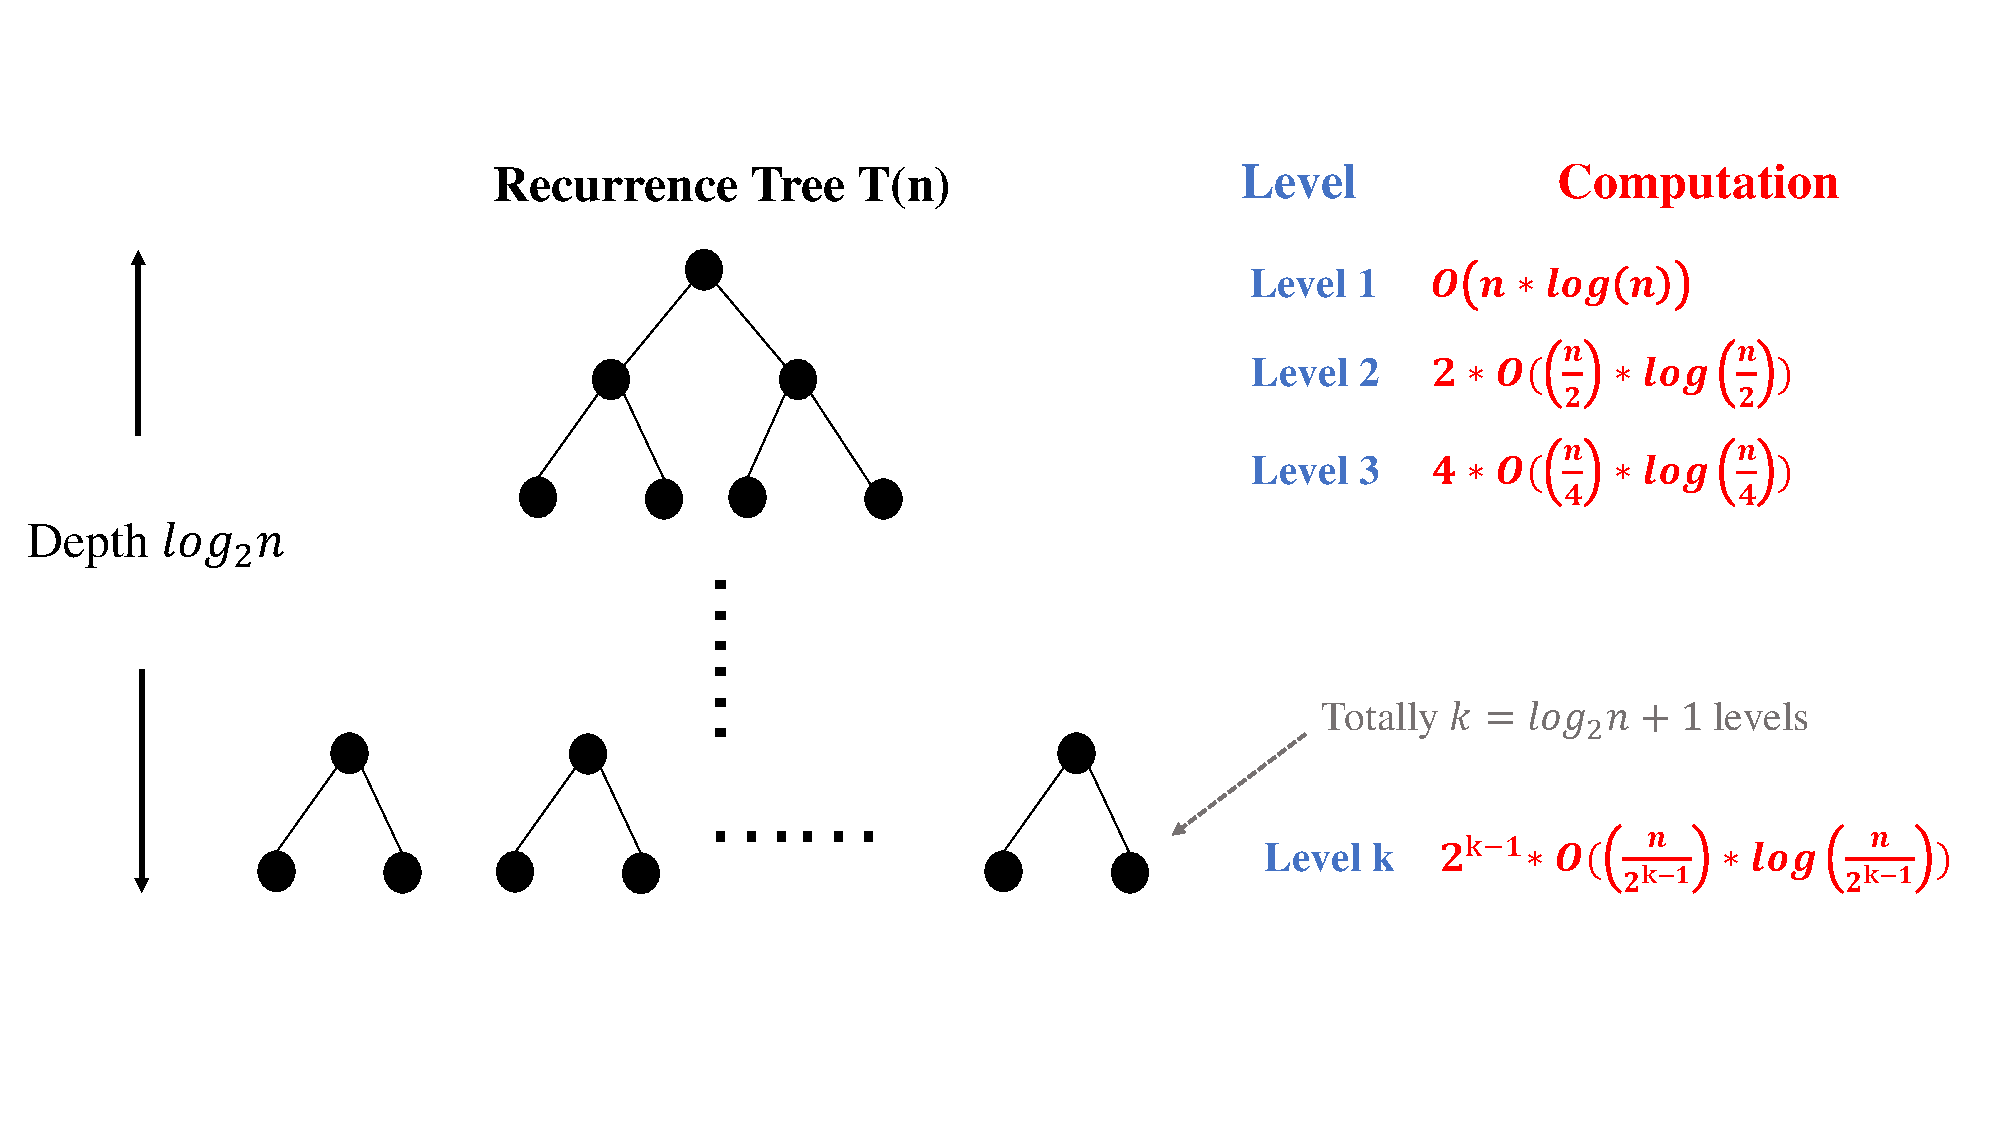
\includegraphics[width=0.8\textwidth]{Fig-RecurrenceTree.pdf}
    \caption{Recurrence Tree}\label{Fig-RecurrenceTree}
\end{figure}
\begin{equation}
    T(n)=\sum_{i=1}^{k} 2^{i-1}O(\frac{n}{2^{i-1}}*log(\frac{n}{2^{i-1}})=\sum_{i=0}^{log  n}O(n*i)=O(n*k^2)=O(n*log^2n)
\end{equation}
\item We are not able to use the typical Master Theorem to solve it.That is because there do not exist a fixed $\epsilon>0$  such that $n*log^2n=\Omega(n^{1+\epsilon})$.
\\Fortunately,we can modify this theorem to 
\begin{equation}
\begin{aligned}
    if~~~~~~~~~~~~~~~~~~~~f(n)=n^{log_b a}*(log^k n)\\
    then~~~~~~~~~~~T(n)=\Theta(n^{log_b a}*(log^{k+1} n))
\end{aligned}
\end{equation}
Then we can from $log_b a=1,f(n)=O(n*logn)$ get $T(n)=\Theta(n^{log_b a}*(log^{2} n))$
\end{enumerate}
\end{solution}
\item
\textit{Transposition Sorting Network.} A comparison network is a \textbf{transposition network}  if each comparator connects adjacent lines, as in the network in Fig.~\ref{Fig-Transposition}.

\begin{figure}[htbp]
    \centering
    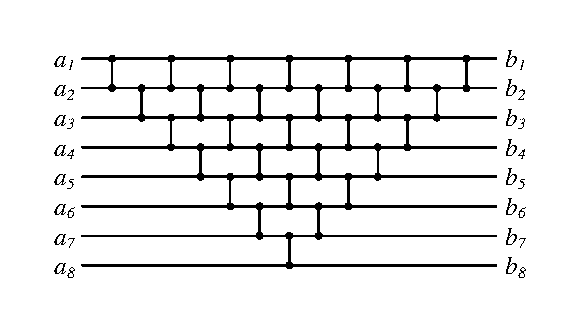
\includegraphics[width=0.4\textwidth]{Fig-Transposition.pdf}
    \caption{A Transposition Network Example}\label{Fig-Transposition}
\end{figure}

\begin{enumerate}
\item Prove that a transposition network with $n$ inputs is a sorting network if and only if it sorts the sequence $\langle n, n-1, \cdots, 1 \rangle$. {\color{blue}(Hint: Use an induction argument analogous to the \emph{Domain Conversion Lemma}.)}
\item {\color{red}{(Optional Sub-question with Bonus)}} Given any $n \in \mathbb{N}$, write a program using Tkinter in Python to draw a figure similar to Fig.~\ref{Fig-Transposition} with $n$ input wires.
\end{enumerate}

\begin{solution}
    ~\par
\begin{enumerate} 
    \item 
    \begin{enumerate}
        \item Necessity is obvious.
        \item Here prove the sufficiency.
        % Transposition Sorting Network is a Sorting Network,so it also satisfies the zero-one principle.That is we only need to prove that if a Transposition Sorting Network can sort reverse ordered sequence, it can solve any 0-1 input situations.\\
        % Basis:when k=1,this is correct obviously.\\
        % Assumptions:for any $n$-element Sorting Network, if it can sort reverse ordered sequence, it can solve any $0-1$ input sequence.\\
        % Induction:There a Transposition Sorting Network can sort reverse ordered sequence.For a random $n+1$ input sequence,if the $(n+1)^{th}$ element is 1,
        \item First of all, we have several definations.\\
        Firstly,We define the time $t$ to be the times the comparators works.If n comparators work in the same depth,we consider it as n time step.For the comparators in the same depth,the less number of wire is in earlier time.  For instance in Figure~\ref{Fig-Transposition}, inputting numbers is in $t=0$,comparing $a_1$ and $a_2$ is in $t=1$,and and comparing $a_3$ and $a_4$ is in $t=4$.\\
        Secondly,We regard the wires from top to bottom as wire 0 to wire 1,which means each time step, if wire $i$ works,it can only compare its output to either $i-1$ or $i+1$.\\
        Thirdly, we define the input sequence as $R$ (random input).Worth to noting that we call the reverse ordered input sequence to be $W$ (worst input).\\
        Lastly, we define the output of the wire$i$ in $t=t_0$ from the input sequence $R$ as $Out_R(i,t_0)$.
        \item Hypothesis:
        \begin{equation}
        \begin{aligned}
            \forall~ 0\le i<j\le n,~~\forall t,~~\forall R~~~~~~~~~~~~~~~~~~~~~~~~~~~~~~~\\
            Out_W(i,t)<Out_W(j,t)\Rightarrow Out_R(i,t)<Out_R(j,t)
        \end{aligned}
        \end{equation}
        \item Basis: \\When $t=0$, $\forall i<j$, $Out_W(i,t)>Out_W(j,t)$,it is obviously correct.
        \item Assumption:\\ When $t=k$, the hypothesis is correct.
        \item Induction:\\
        Assume this time comparator works between wire $m$ and $m+1$,and $Out_R(i,t+1)<Out_R(j,t+1)$.\\
        1)$i<m,j>m+1$
        \begin{equation}
            \begin{aligned}
            &Out_W(i,t)=Out_W(i,t+1)<Out_W(j,t+1)=Out_W(j,t)\\
            \Rightarrow& Out_R(i,t)=Out_R(i,t+1)<Out_R(j,t+1)=Out_R(j,t)
            \end{aligned}
        \end{equation}
        2) $i=m,j=m+1$.\\
        From the defination of the comparator we know no matter how large is $Out_W(i,t)$ and $Out_W(j,t)$, there must be $Out_R(i,t+1)<Out_R(j,t+1)$.\\
        3) $i<m,j=m$.
        \begin{equation}
                Out_W(i,t)=Out_W(i,t+1)<Out_W(j,t+1)=min\{Out_W(m,t),Out_W(m+1,t)\}
            \label{2}
        \end{equation}
        From equation~\ref{2} we can get:
        \begin{equation}
                 Out_R(i,t+1)=Out_R(i,t)<min\{Out_R(m,t),Out_R(m+1,t)\}=Out_R(m,t+1)
        \end{equation}
        4)$i<m,j=m+1$
        \begin{equation}
            Out_W(i,t)=Out_W(i,t+1)<Out_W(j,t+1)=max\{Out_W(m,t),Out_W(m+1,t)\}
            \label{3}
        \end{equation}
        From equation~\ref{3} we can get:
        \begin{equation}
            \begin{aligned}
            Out_R(i,t+1)=Out_R(i,t)<max\{Out_R(m,t),Out_R(m+1,t)\}=Out_R(m+1,t+1)
            \end{aligned}
        \end{equation}
        5)$i=m+1,j>m+1$ 
       \begin{equation}
                Out_W(j,t)=Out_W(j,t+1)>Out_W(i,t+1)=max\{Out_W(m,t),Out_W(m+1,t)\}
            \label{4}
        \end{equation}
        From equation~\ref{4} we can get:
        \begin{equation}
                 Out_R(j,t+1)=Out_R(j,t)>max\{Out_R(m,t),Out_R(m+1,t)\}=Out_R(i,t+1)
        \end{equation}
        6)$i=m,j>m+1$ 
       \begin{equation}
                Out_W(j,t)=Out_W(j,t+1)>Out_W(i,t+1)=min\{Out_W(m,t),Out_W(m+1,t)\}
            \label{5}
        \end{equation}
        From equation~\ref{5} we can get:
        \begin{equation}
                 Out_R(j,t+1)=Out_R(j,t)>min\{Out_R(m,t),Out_R(m+1,t)\}=Out_R(i,t+1)
        \end{equation}
        So when $t=k+1$, the hypothesis is correct.
        \item From the mathematical induction theorem,we can get the conclusion that
        \begin{equation}
        \begin{aligned}
            \forall~ 0\le i<j\le n,~~\forall t,~~\forall R~~~~~~~~~~~~~~~~~~~~~~~~~~~~~~~\\
            Out_W(i,t)<Out_W(j,t)\Rightarrow Out_R(i,t)<Out_R(j,t)
        \end{aligned}
        \end{equation}
        As a result, if a Transposition Network can sort input $W$,we assume it ends at $t=t_0$.This time,$\not\exists i<j, Out_W(i,t_0)<Out_W(j,t_0)$.From the proof we know ,$\not\exists i<j, Out_R(i,t_0)<Out_R(j,t_0)$, which means the random input $R$ is sorted. So this is a Sorting Network.  
    \end{enumerate}
    \item Python code is in appendix 2.\\The results are in the Figure~\ref{fig:my_label1}
    \begin{figure}
        \centering
        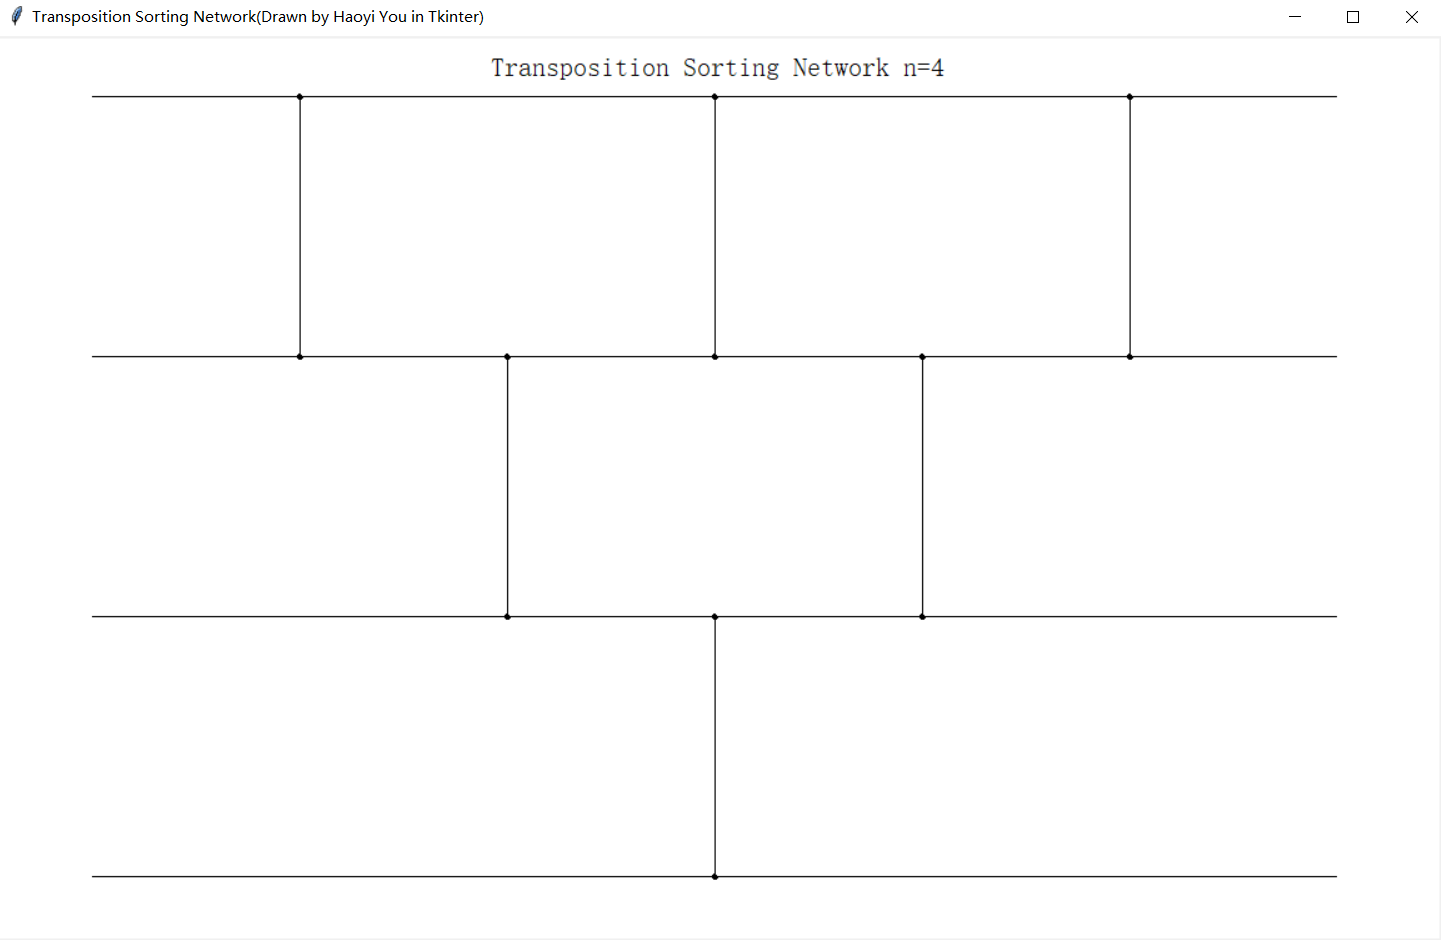
\includegraphics[width=0.45\textwidth]{n=4.png}
        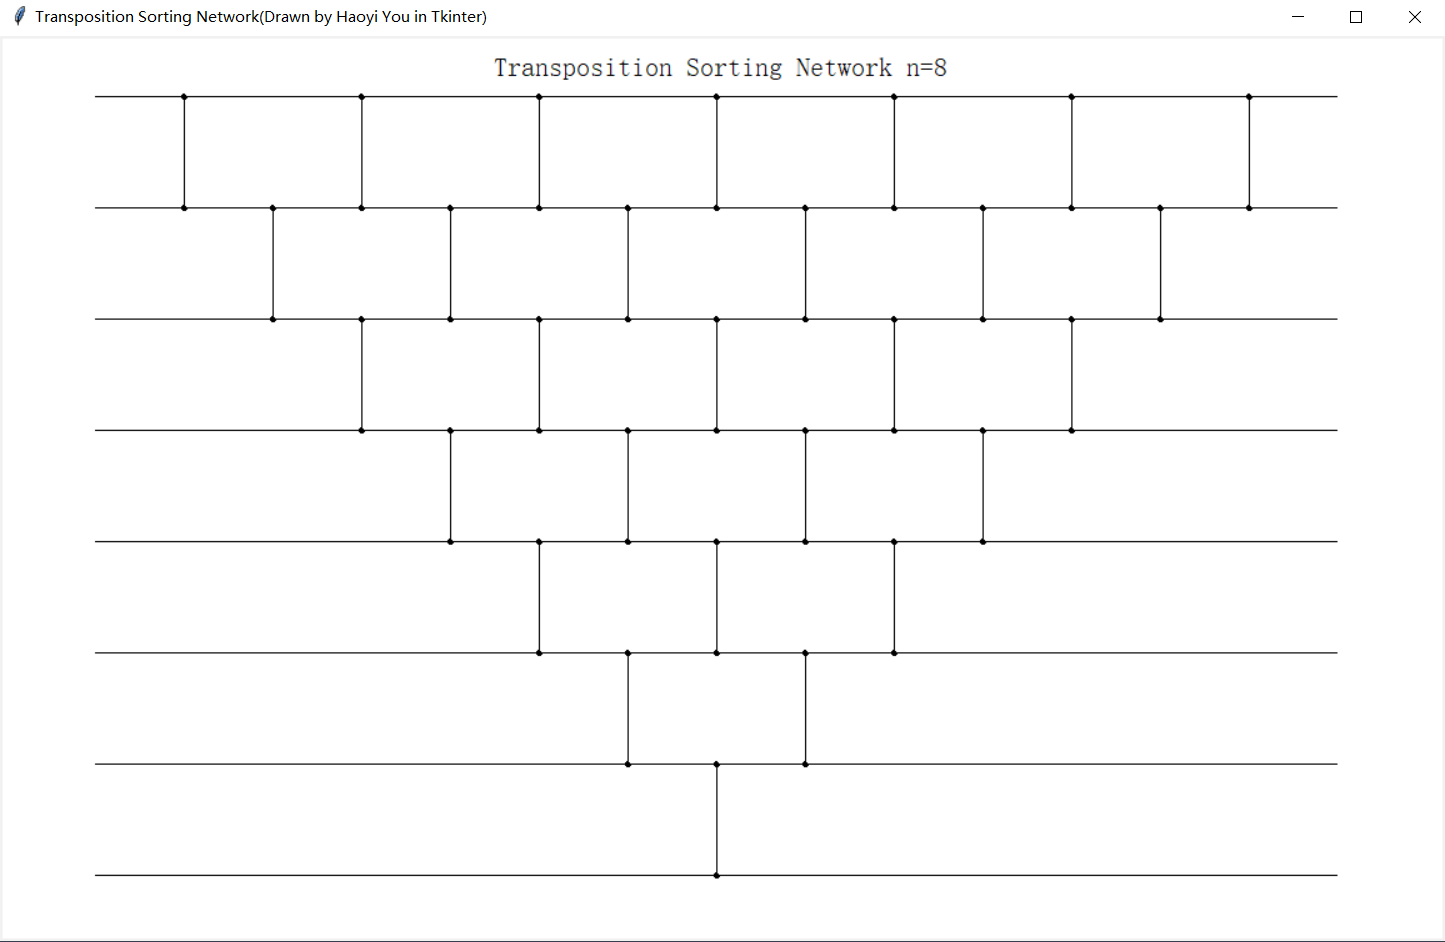
\includegraphics[width=0.45\textwidth]{n=8.png}
        \\
        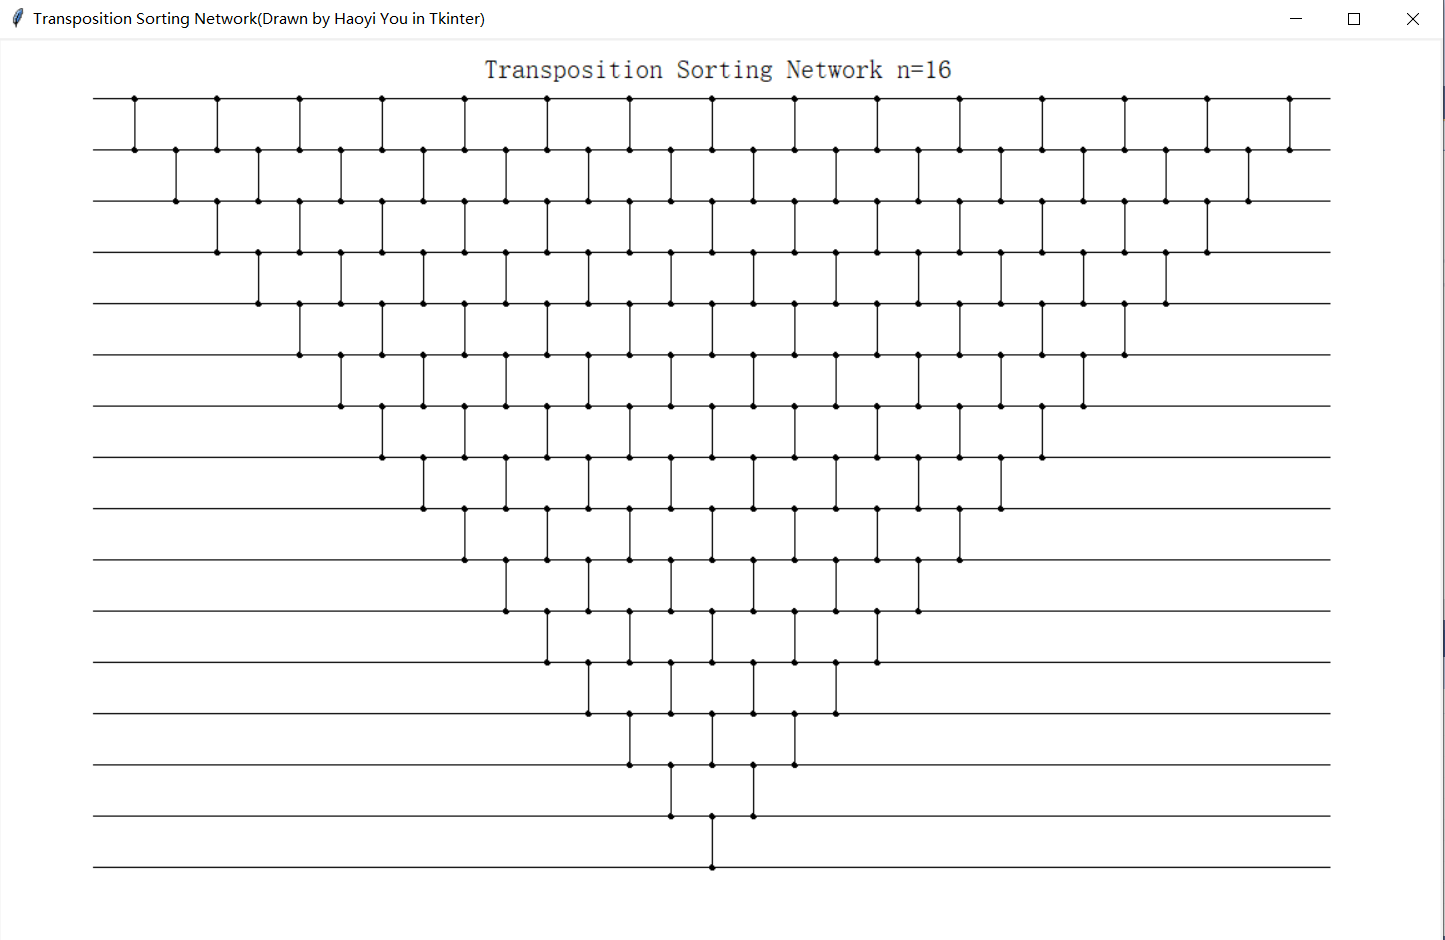
\includegraphics[width=0.45\textwidth]{n=16.png}
        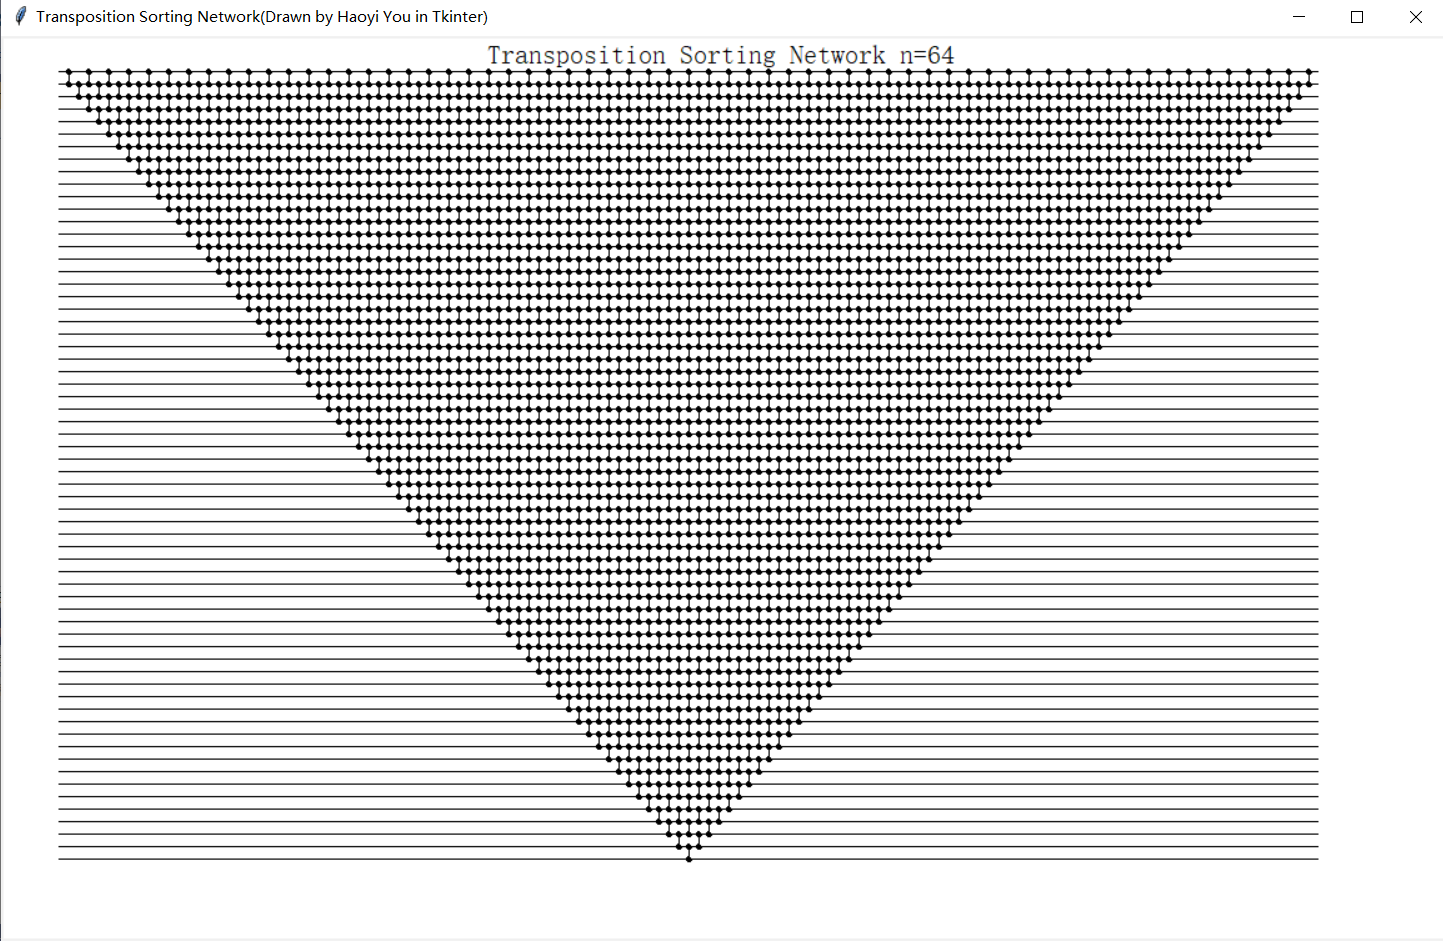
\includegraphics[width=0.45\textwidth]{n=64.png}
        \caption{Transposition Network with various n}
        \label{fig:my_label1}
    \end{figure}
\end{enumerate}

\end{solution}
\end{enumerate}
\clearpage
%========================================================================
\appendix
\section{Appendice}
\subsection{C++ code for problem 2}
\begin{lstlisting}[language=C++,numberstyle=\tiny, 
        basicstyle=\small]
#include <iostream>
#include <vector>
#include <algorithm>
using namespace std;

int binary_search_for_m(vector<long>& sum, long sum_i, int LOWER, int low, int high) {
	if (high <= low|| sum[high-1] - sum_i < LOWER)return high;
	int min = low, max = high-1, mid;
	while (min<max) {
		mid = (max + min) / 2;
		if (sum[mid] - sum_i >= LOWER)max = mid;
		else min = mid+1;
	}
	return max;
}

int binary_search_for_n(vector<long>& sum, long sum_i, int UPPER, int low, int high) {
	if (high <= low || sum[high-1] - sum_i <=UPPER)return high;
	int min = low, max = high - 1, mid;
	while (min < max) {
		mid = (max + min) / 2;
		if (sum[mid] - sum_i > UPPER)max = mid;
		else min = mid + 1;
	}
	return max;
}

int merge_count(vector<long>& sum, int low, int high, int LOWER, int UPPER) {
	int mid = (low + high) / 2;
	if (mid == low)
		return 0;
	int count = merge_count(sum, low, mid, LOWER, UPPER)
		+ merge_count(sum, mid, high, LOWER, UPPER);
	int m_low = mid, m_high = high, n_low = mid, n_high = high;
	for (int i = low; i < mid; i++) {
		int m = binary_search_for_m(sum, sum[i], LOWER, m_low, m_high);
		int n = binary_search_for_n(sum, sum[i], UPPER, n_low, n_high);
		count += n - m;
	}
	sort(sum.begin() + low, sum.begin() + high);
	return count;
}

int main() {
	int N, LOWER, UPPER;
	vector<int> A;
	vector<long> sum(1, 0);

	cin >> N >> LOWER >> UPPER;
	for (int tmp, i = 0; i < N; i++) {
		cin >> tmp;
		A.push_back(tmp);
		sum.push_back(sum.back() + A.back());
	}

	cout << merge_count(sum, 0, N + 1, LOWER, UPPER) << endl;

	return 0;
}
\end{lstlisting}
\subsection{Python code for problem 3}
\begin{lstlisting}[language=Python,numberstyle=\tiny, 
        basicstyle=\small]
from tkinter import *

class MyCanvas(Canvas):
    def __init__(self, master, hLineWidth=1, vLineWidth=1, radius=2, **kwargs):
        Canvas.__init__(self, master, kwargs)
        self.hLineWidth = hLineWidth
        self.vLineWidth = vLineWidth
        self.radius = radius

    def create_segment_h(self, x, y, l):
        self.create_line(x, y, x + l, y, width=self.hLineWidth)
        self.create_oval(x - self.radius, y - self.radius, x + self.radius,
        y + self.radius, fill='black')
        self.create_oval(x + l - self.radius, y - self.radius, x + l - self.radius,
        y + self.radius, fill='black')

    def create_segment_v(self, x, y, l):
        self.create_line(x, y, x, y + l, width=self.vLineWidth)
        self.create_oval(x - self.radius, y - self.radius, x + self.radius, 
        y + self.radius, fill='black')
        self.create_oval(x - self.radius, y + l - self.radius, x + self.radius, 
        y + l + self.radius, fill='black')

    def create_line_h(self, x, y, l):
        self.create_line(x, y, x + l, y, width=self.hLineWidth)

    def create_line_v(self, x, y, l):
        self.create_line(x, y, x, y + l, width=self.vLineWidth)

    def text(self,string,x,y):
        self.create_text(x, y,font=('Pursia',16),text=string)


class Draw:
    def __init__(self, size):
        self.size=size
    def hNum(self):
        return 1
    def draw(self, cvs, x, y, hScale, vScale):
        for i in range(self.size+1):
            cvs.create_line_h(x, y + i * vScale, 2*(self.size) * hScale)
        for i in range(self.size):
            for j in range(self.size-i):
                cvs.create_segment_v(x+(i+1+2*j)*hScale,y+i*vScale,vScale)

if __name__ == '__main__':
    k = int(input('please input the number k: '))
    n = 2 ** k-1

    winW, winH = 1920*0.6, 1200 * 0.6
    hMargin, vMargin = winW // 10, winH // 10
    hScale, vScale = (winW - 2 * hMargin) // (2*n), (winH - 2 * vMargin) // (n)

    root = Tk()
    root.title('Transposition Sorting Network(Drawn by Haoyi You in Tkinter)')
    cvs = MyCanvas(root, bg='white', width=winW, height=winH)
    paint= Draw(n)
    string="Transposition Sorting Network n={}".format(n+1)
    paint.draw(cvs, hMargin, vMargin, hScale, vScale)
    cvs.text(string,winW/2,vMargin/2)
    cvs.pack()

    root.mainloop()

}
\end{lstlisting}
\end{document}
